% ---------------------------------------------------------------------------
% IT5006 Fundamentals of Data Analytics
% Group Project Milestone 2: Analytics Implementation
%   Problem Definition, Model Building and Evaluation
%
% Compiles with pdfLaTeX. Build: pdflatex -> bibtex -> pdflatex x2
% Overleaf: upload the whole report/ folder and set this file as the main
% document; figures/ and refs.bib are picked up from their relative paths.
%
% Every number in this document is regenerated by src/phase2_stats.py into
% report/stats_phase2.txt. Diff the two before submitting.
% ---------------------------------------------------------------------------
\documentclass[11pt,a4paper]{article}

\usepackage{lmodern}      % scalable Type 1 font; required for microtype expansion
\usepackage[T1]{fontenc}
\usepackage[utf8]{inputenc}
\usepackage[margin=1in]{geometry}
\usepackage{graphicx}
\usepackage{booktabs}
\usepackage{longtable}
\usepackage{caption}
\usepackage{subcaption}
\usepackage{amsmath}
\usepackage{tikz}
\usetikzlibrary{arrows.meta,positioning,fit,backgrounds}
\usepackage{microtype}
\usepackage{xcolor}
\usepackage[numbers,sort&compress]{natbib}
\usepackage[hidelinks]{hyperref}

\graphicspath{{figures/}}
\captionsetup{font=small,labelfont=bf,skip=5pt}
\setlength{\parskip}{0.18em}
\setlength{\textfloatsep}{10pt plus 2pt minus 2pt}
\setlength{\intextsep}{10pt plus 2pt minus 2pt}
\bibliographystyle{plainnat}

% Footnotes lettered, with a visible rule, so the notes read as marginal
% commentary rather than as numbered citations.
\renewcommand{\thefootnote}{\alph{footnote}}
\renewcommand{\footnoterule}{\vspace*{4pt}\hrule width 0.45\columnwidth height 0.4pt\vspace*{4pt}}
\makeatletter
\renewcommand\@makefntext[1]{\parindent 1em\noindent\hb@xt@1.4em{\hss\@makefnmark}\footnotesize #1}
\makeatother

% Citation marks a little smaller than body text.
\let\oldcitep\citep
\renewcommand{\citep}[1]{{\footnotesize\oldcitep{#1}}}
\let\oldcitet\citet
\renewcommand{\citet}[1]{{\footnotesize\oldcitet{#1}}}

\newcommand{\code}[1]{\texttt{\small #1}}
% Winning entries in the results tables. Bold alone is ambiguous when a table
% carries both a per-family best and an overall best.
\newcommand{\best}[1]{\textbf{#1}}

% ---------------------------------------------------------------------------
\begin{document}

% ============================== COVER PAGE =================================
\begin{titlepage}
\centering
\vspace*{3.5cm}

{\Large\bfseries Group Project Milestone 2:\par}
\vspace{0.6em}
{\Large\bfseries Analytics Implementation --- Problem Definition,\\[2pt]
Model Building and Evaluation\par}

\vspace{1.2cm}
{\large Predicting Delivery Performance and Satisfaction Risk\par}
\vspace{0.4em}
{\normalsize Two prediction moments on the Olist Brazilian e-commerce marketplace\par}

\vspace{3.5cm}

{\large\bfseries Group 10\par}
\vspace{0.9em}

{\normalsize
\begin{tabular}{@{}l@{\hspace{1.5em}}l@{}}
Pan Pinyou  & A0329105L \\[3pt]
Li Yudan    & A0330335R \\[3pt]
Zhu Gengyu  & A0333773Y \\
\end{tabular}\par}

\vfill

{\large National University of Singapore\par}
\vspace{0.4em}
{\large IT5006 Fundamentals of Data Analytics\par}
\vspace{0.4em}
{\large AY2026/2027 Semester 1\par}

\vspace{1.1cm}
{\normalsize
\textbf{Dashboard:} \url{https://team10-it5006-olist.streamlit.app}\\[4pt]
\textbf{Repository:} {\small\url{https://github.com/gengyuzccc-cell/Team10_IT5006_Ecommerce_Analytics_AY2627Sem1}}\par}

\vspace{1.2cm}
\end{titlepage}

% ============================== BODY =======================================
\section{Problem Definition and Stakeholder Context}
\label{sec:problem}

Phase 1 left one finding standing above the rest: a late delivery raises the
probability of a 1--2 star review from 9.2\% to 54.0\%, a 5.9-fold increase
monotone in how late the parcel is. Phase 2 turns that sentence into a pair of
predictions placed at two points in an order's life.

\begin{table}[htbp]
\centering
\caption{The two problems. They share one feature pipeline, one model-family
budget and one dataset; what separates them is \emph{when} the model runs.}
\label{tab:problems}
\small
\begin{tabular}{@{}p{1.9cm}p{6.2cm}p{6.2cm}@{}}
\toprule
 & \textbf{Problem 1 --- delivery performance} & \textbf{Problem 2 --- satisfaction risk} \\
\midrule
Question & How long will this order take, and will it miss its promise? &
Will this delivered order draw a 1--2 star review? \\[2pt]
Moment & \code{at\_checkout} --- the order has just been placed &
\code{at\_delivery} --- the parcel has arrived, the review is not yet written \\[2pt]
Stakeholder & Operations and logistics & Customer experience \\[2pt]
Task & \textbf{1A regression}: lead time in days, on MAE.
\textbf{1B classification}: delivered after the promised date, on PR-AUC against
its no-skill floor &
\textbf{Classification}: \code{review\_score} $\le 2$, on PR-AUC against its
floor and balanced accuracy \\[2pt]
Action & Re-quote the promise, warn the buyer, expedite freight &
Reach out before the review lands \\
\bottomrule
\end{tabular}
\end{table}

The brief permits two problems or one framed twice; we take two, because they are
halves of one decision chain. Operations acts before the parcel ships; customer
experience acts after it arrives and before the customer writes anything.
Problem 1's output is, in substance, Problem 2's most important input.

Problem 1 is the brief's \emph{dual framing}: one underlying quantity, two
outputs, so the late-order flag \emph{is} the regression's answer compared
against the promised date. Five classifiers trained directly on the binary label
run alongside as a control arm, testing whether the flag needs a model of its
own; Section~\ref{sec:results-late} reports that comparison, including a
disagreement between the selection protocol and the forward window that is itself
one of this report's findings.

\paragraph{Targets.} All three come from the provided tables alone.
\emph{Lead time} is \code{order\_delivered\_customer\_date} $-$
\code{order\_purchase\_timestamp} in days, defined for the 97.0\% of orders that
reached the customer. \emph{Late} is delivery strictly after
\code{order\_estimated\_delivery\_date}, which carries no time component, so
lateness is accurate to about a day. \emph{Low review} is \code{review\_score}
$\le 2$, defined for the 99.2\% carrying a review. Undefined rows are \code{NaN}
and excluded, never imputed to a negative label: the event has not happened
rather than gone missing, and a silent customer is not a satisfied one.

\paragraph{Success criteria, registered in advance.}
Expected ranges for all six headline metrics were written into
\code{config.EXPECTED\_BANDS} \emph{before} any Phase 2 model was tuned, from the
Phase 1 results and untuned scoping probes (Appendix~\ref{app:bands}). They are
the targets the work is judged against and they are a leak alarm --- because here
the signature of leakage is not a subtle improvement but an implausible one, as
Phase 1 showed by adding one forbidden column to the late-delivery model and
watching ROC-AUC go from 0.589 to 1.000. A result landing far \emph{above} its
band is investigated before it is reported. All six landed inside; none above.

The ceiling deserves stating as plainly as the target: lateness here is volatile
rather than trending --- 1.4\% to 21.4\% month to month with Black Friday
congestion and the May 2018 truckers' strike --- and no order-level feature
available at checkout can anticipate a national road blockade. A late-delivery
classifier reporting 95\% accuracy here would be the majority-class rule or a
leak.

\section{Data Preparation and Feature Engineering}
\label{sec:data}

\subsection{From nine tables to one row per order, split three ways}

The preparation pipeline is inherited unchanged from Phase 1
(\code{src/data\_load.py}). Three of the nine source tables --- items, payments
and reviews --- are one-to-many against orders, so each is aggregated to the
order grain \emph{before} joining; a direct merge yields 118{,}437 rows rather
than 99{,}441 and silently reweights every mean towards large baskets. The grain
is asserted after the join, and \code{customer\_unique\_id} is carried throughout
because \code{customer\_id} is regenerated per order and is not a person.
Restricting to the fully-operational window leaves \textbf{99{,}091} orders.
Eleven cleaning decisions with their evidence are recorded as
\code{CLEANING\_DECISIONS} in the loader and tabulated in the Phase 1 appendix;
\code{src/report\_stats.py} still reproduces every Phase 1 number byte-for-byte
after the Phase 2 additions, which \code{tests/test\_leakage.py} asserts.

Each period has exactly one job. \textbf{Train} (2017-01-01\,--\,2018-04-30,
73{,}008 orders) fits every model, with expanding-window cross-validation inside
it tuning hyperparameters. \textbf{Validation} (2018-05-01\,--\,2018-06-30,
13{,}156) sets every decision threshold and fits the margin-to-risk calibration.
\textbf{Test} (2018-07-01\,--\,2018-08-31, 12{,}927) is scored once, at the end,
for models already chosen. The split is chronological rather than
stratified-random because the target drifts, and additionally disjoint on the
customer: 2{,}997 people ordered more than once, so a purely temporal cut can
still put one of a person's orders on each side, and the \textbf{227} straddling
buyers are removed from a clean test subset used in
Section~\ref{sec:results-review}.

\subsection{Features, and the moment each becomes knowable}

Phase 1's 25 features carry forward unchanged: 6 calendar (month, weekday, hour,
weekend, business hours, the Black Friday window), 11 basket-and-money
(\code{log\_price}, \code{freight\_ratio}, \code{log\_weight}, volume, item and
seller counts, instalments), 4 geographic (\code{log\_distance},
\code{same\_state}, customer state, seller region), 2 for the promise and 2
catalogue. The design carries no exact duplicates --- Phase 1's first draft held
\code{total\_price} alongside \code{log\_price} and \code{total\_payment}, which
makes a linear baseline meaningless --- and \code{purchase\_year} is absent
because the split is chronological, so a linear term on it would extrapolate into
an unseen year. Phase 2 adds \textbf{eight track-record features}, taking the
checkout set to 33 and the at-delivery set to 36: a seller's mean lead time, late
rate, low-review rate and order count; a route's mean lead time; a category's
low-review rate; and the platform's own lead time and late rate. The at-delivery
regime additionally sees three columns describing how delivery actually went.

\paragraph{Why these features.}
Phase 1 chose the feature groups from the structure of the data; the Milestone 1
feedback asked for the literature behind them. \emph{Geography:}
origin--destination structure and distance are the backbone of published
delivery-time models, from JD.com's arrival forecasts \citep{salari2022delivery}
to last-mile travel-time predictors \citep{liu2021lastmile}. \emph{The promise:}
the quoted date is itself a decision that encodes what the platform's routing
knew \citep{cui2024promise, salari2022delivery}, which is why it is admissible
and useful at checkout. \emph{Basket, money and calendar:} order size, value and
freight are the order-level controls through which \citet{deshpande2023logistics}
identify the logistics--rating link, and demand peaks stress fulfilment
\citep{cui2024promise}, which Section~\ref{sec:problem} measures for Black
Friday. \emph{Track records:} the past performance of the parties to a
transaction is the standard predictor in supply-chain delay models
\citep{baryannis2019risk}, and an as-of aggregate of a key's earlier outcomes is
the time-respecting form of target encoding \citep{miccibarreca2001target}; the
general vocabulary of counts, ratios and calendar encodings follows
\citet{kuhn2019feature} and \citet{heaton2016feature}. The empirical screen was
Phase 1's correlation matrix (its Figure~8): lead time correlates 0.39 with
distance, 0.38 with the promised window, 0.17 with freight and 0.07 with weight;
promise and distance correlate 0.52 with each other, so both are kept and the
trees resolve the overlap; and the review score correlates $-0.33$ with lead
time and essentially zero with price or basket size -- the delivery, not the
purchase, drives the rating.

\subsection{Track records, and the trap inside them}
\label{sec:history}

A seller's history is the strongest thing a marketplace knows about an order at
checkout, and the easiest place here to leak, because of a distinction that is
easy to miss: \emph{past} means the earlier order had \textbf{closed} before this
one was placed --- not merely that it was placed earlier. A parcel bought last
week that has not yet arrived has no lead time yet, so ordering the history by
\emph{purchase} time would let every order average in outcomes that had not
happened. That is Kaufman et al.'s \emph{illegitimate feature}
\citep{kaufman2012leakage} in a convincing disguise, and it would be invisible in
the metrics because it would simply look like a better model. Every aggregate is
therefore an as-of join against the moment the earlier outcome became observable
--- \code{order\_delivered\_customer\_date} for delivery,
\code{review\_creation\_date} for reviews --- with a strict boundary.

Two further guards. A mean over one previous order is noise rather than a rate,
so below a floor of five prior orders the value is undefined and a fallback chain
takes over (seller $\rightarrow$ route $\rightarrow$ seller state $\rightarrow$
platform), after which 0.95\% of orders lack any history value. And cold start is
information rather than error: \code{hist\_seller\_n} carries how many past
orders the estimate rests on, so a model can discount a seller it has barely
seen. The platform features additionally use a \textbf{28-day trailing window}
rather than an expanding mean --- lead time halves across the analysis window, so
an average over all history reports roughly 13 days while the current month runs
at 8 --- and their range, 5.2 to 17.1 days, is a direct measure of the drift the
models must survive.

Because a leak here would be invisible in the metrics, the construction is
checked rather than reviewed: \code{tests/test\_leakage.py} rebuilds
\code{hist\_seller\_lead\_days} from first principles for 200 random orders and
requires exact agreement, and a second check confirms the platform tracker
\emph{lags} rather than anticipates (Appendix~\ref{app:repro}).

\subsection{Leakage: one rule per prediction moment}

Leakage here is not one rule but one per \emph{prediction moment}, because what
is known depends on when the model runs. \emph{At checkout} nothing about
fulfilment or the customer's opinion exists, so delivery dates and everything
derived from them, the review score and its timestamps,
\code{order\_approved\_at}, \code{shipping\_limit\_date} and
\code{order\_status} are forbidden. \emph{At delivery} only the review and its
timestamps remain forbidden --- the delivery outcome is now history, and the
brief itself lists ``delivery performance'' among the features for that problem.
\code{assert\_no\_leakage(features, regime)} enforces the correct set before any
model is fitted, is tested in both directions, and raises on an unrecognised
regime name, because passing the wrong regime is itself the mistake it exists to
catch.

\code{order\_estimated\_delivery\_date} is admissible at checkout and matters:
the customer is shown that promise when the order is placed, so it precedes the
outcome and encodes whatever Olist's own routing knew. It is a useful feature and
--- Section~\ref{sec:results-reg} --- a poor prediction. The cost of getting the
regime wrong is measurable: adding one forbidden column, the realised delivery
time, lifts the late-delivery model's ROC-AUC from 0.589 to \textbf{1.000}. That
is not a result; it is the target restated.

\section{Modelling Methodology}
\label{sec:method}

\subsection{Model family budget and pipelines}

The brief allows two to three families and asks for depth rather than breadth. We
use three, reused across both task types, each arranged as a \emph{complexity
ladder} whose rung 0 is the family's simplest variant --- which is the only way
``the added complexity was worth it'' becomes a finding rather than an
assumption. \textbf{A --- Linear} runs \code{LinearRegression} /
\code{LogisticRegression} at rung 0 and \code{Ridge} / $\ell_2$-penalised
logistic at rung 1. \textbf{B --- Tree-based} runs \code{DecisionTree} $\to$
\code{RandomForest} $\to$ \code{HistGradientBoosting}. \textbf{C --- Ensemble} is
soft \code{Voting} and \code{Stacking} assembled from the winners of A and B; its
members are complete pipelines rather than bare estimators, because the two
families need different encodings and one shared preprocessor would force a
single choice on both. The full specification, search spaces and selected values
are in Appendix~\ref{app:hyperparameters}.

\paragraph{Why these rungs, from the literature rather than from our results.}
The Milestone 1 feedback observed that Phase 1 cited the original algorithm
papers and compared families only broadly, so the rungs are argued here before
any result is shown. Within family B they are the three ways the literature
knows to improve on one tree: a random forest bags decorrelated trees to cut
variance \citep{breiman2001rf}; boosting fits trees to residuals with shrinkage
to cut bias \citep{friedman2001gbm}. Across the large empirical comparisons --
ten algorithms on eleven problems \citep{caruana2006empirical}, 179 classifiers
on 121 datasets \citep{fernandezdelgado2014hundreds}, 45 tabular benchmarks
against deep architectures \citep{grinsztajn2022tabular, shwartzziv2022tabular}
and 41 classifiers on business credit data \citep{lessmann2015benchmarking} --
boosted and bagged tree ensembles are the consistent top tier, boosting usually
ahead by a small margin. The boosted learner is \code{HistGradientBoosting}
rather than a third-party library because it is LightGBM's histogram-binned
design \citep{ke2017lightgbm} implemented inside \code{scikit-learn}
\citep{sklearn2024hgb}, so it stays within the brief's toolset; because it
handles missing values natively, which the cold-start track-record features
need; and because it fits an order of magnitude faster than a comparable
forest, which made a 30-draw search affordable. In e-commerce and logistics the
same family is the working choice -- quantile regression forests for delivery
times at JD.com \citep{salari2022delivery}, tree models for late supplier
deliveries \citep{baryannis2019risk}, and random forests or boosted trees in
the published studies on this very dataset \citep{fouad2023satisfaction,
wangkiat2023satisfaction, gopinadh2025satisfaction}, none of which controls
leakage by prediction moment, the gap Section~\ref{sec:data} closes. The ladder
then supplies what the literature cannot: on this data each rung must beat the
one below it, and Section~\ref{sec:results} reports where it does not.

Every model is a \code{scikit-learn} \code{Pipeline}: median imputation, one-hot
encoding of the four categoricals with rare levels folded into one bucket, then
--- for the linear family only --- standardisation, since trees are invariant to
monotone rescaling and a shared penalty is not \citep{pedregosa2011sklearn}. The
linear family additionally drops one level per categorical. That is a
correction rather than a preference: Phase 1 reported that ordinary least
squares was unusable here, ``rank-deficient, so its coefficients explode'', and
re-running it four ways (Appendix~\ref{app:encoding}) shows the predictions were
always fine (test MAE 4.181, indistinguishable from Ridge) and only the
coefficient vector was not; dropping a level restores full rank, after which
Ridge and OLS agree to three decimals. Regularisation buys numerical stability
here, not accuracy.

\subsection{Cross-validation, and how a model gets chosen}
\label{sec:cv}

Delivery performance drifts hard --- mean lead time falls \textbf{5.34 days}
between training and test --- so shuffled $k$-fold lets a model learn from the
future, the invalidity \citet{bergmeir2012cv} formalise. Hyperparameters are
tuned by \code{TimeSeriesSplit} with five expanding windows inside the training
period, searched with \code{RandomizedSearchCV} \citep{bergstra2012random} over
30 draws per model --- six for the random forests, which cost one to two orders
of magnitude more per fit --- scoring \code{neg\_mean\_absolute\_error} for
regression and \code{average\_precision} for classification.

\emph{Selecting} between tuned models is a separate question, and both obvious
answers fail here for reasons that are properties of the data. Averaging
cross-validated scores fails because the folds differ enormously in difficulty
--- lead time runs 12--17 days across the 2017 folds against 8.3 in the test
window --- so every model's CV error sits about a day above its forward error and
the \emph{ordering} does not survive: cross-validated MAE ranks Ridge above the
boosted trees, while every later window and the test period rank them the other
way round. Using the validation period alone fails too: two months is short, and
these two pull in opposite directions, the late rate being 8.2\% in May 2018 and
\textbf{1.4\%} in June, the lowest in the series.

Each candidate is therefore scored on all six out-of-sample windows ---
the five expanding folds and the validation period --- \textbf{ranked within
each}, and the winner is the best mean rank over the \textbf{three most recent}.
Ranks rather than scores, because ranks are the only thing comparable across
windows of different difficulty and different base rates; three windows because
that covers roughly February to June 2018, recent enough to resemble deployment
and wide enough that neither of the validation period's two odd months decides
alone. All six are reported in \code{report/results/selection\_*.csv}. A
shuffled, customer-disjoint \code{StratifiedGroupKFold} is computed alongside as
a contrast exhibit and never used to choose anything. The selected models are
\emph{not} refitted on train plus validation before the test window is scored: a
production system should, but that would decouple the shipped artifact from the
threshold and calibration fitted against it, and what is reported here is exactly
what is deployed. What the two cross-validation protocols would have reported,
and why their raw PR-AUC is not comparable with the forward window, is
quantified in Appendix~\ref{app:protocol}.

\subsection{Imbalance, metrics aligned to the action, and reproducibility}
\label{sec:imbalance}

Both targets are imbalanced --- 7.4\% late and 11.0\% low review in the test
period --- so accuracy alone is meaningless and every results row carries
\code{majority\_accuracy} beside \code{accuracy}, with PR-AUC reported against
its no-skill floor \citep{saito2015prplot}. Phase 1's literature review argued
from \citet{goorbergh2022imbalance} that correcting imbalance does not improve
discrimination and badly miscalibrates the result, and committed Phase 2 to
testing rather than assuming it (Section~\ref{sec:results-review}). We fit on the
observed prior and move the \emph{decision threshold} instead, tuned on the
validation period by maximising F1 --- which changes the decision without
distorting the probability. Calibrated probabilities are a requirement rather
than a nicety, because Section~\ref{sec:cost} multiplies them by a cost
\citep{elkan2001cost}; they are reported, not assumed
\citep{niculescu2005calibration}. No resampling is used anywhere.

A second alignment follows from Table~\ref{tab:levers}. PR-AUC summarises the
whole ranking and is the right criterion for \emph{choosing} between models,
but neither team acts on the whole ranking: customer experience contacts the
$K$ riskiest deliveries its agents can reach in a day, and operations reviews
the top of the late list. The quantity that describes their day is the precision
and recall of that top-$K$ -- the targeting view of \citet{provost2013data},
and the top-decile lift that profit-driven evaluation uses in place of accuracy
\citep{verbeke2012churn, lessmann2015benchmarking}.
Section~\ref{sec:results-capacity} therefore reports Precision@$K$ and
Recall@$K$ for both flags, with $K$ as a share of the day's volume so that the
same table holds on a quiet Tuesday and on Black Friday, and
Section~\ref{sec:cost} chooses the operating point as a capacity rather than
as a threshold.

\code{SEED = 42} throughout. \code{src/train\_models.py} fits everything and
writes the models, metadata and every result table; \code{src/phase2\_stats.py}
distils those into \code{report/stats\_phase2.txt}, and no number enters this
report that it cannot regenerate. Every figure is drawn from those same tables,
so a figure cannot disagree with one. Artifacts record the \code{scikit-learn}
version that wrote them and the loader checks it;
\code{tests/test\_leakage.py} runs 41 validation checks
(Appendix~\ref{app:repro}).

\section{Results}
\label{sec:results}

Everything below is the untouched test window, 2018-07-01 to 2018-08-31, scored
once for models already chosen. Cross-validated and validation columns sit beside
it because the disagreement between them is part of the result. Figures are in
Appendix~\ref{app:figures}.

\subsection{Problem 1A --- lead time}
\label{sec:results-reg}

\begin{table}[htbp]
\centering
\caption{Lead-time regression: two reference points that are not models, then
each family's complexity ladder. \best{Bold} is the selected model.
Figure~\ref{fig:ladder}.}
\label{tab:reg}
\small
\begin{tabular}{@{}llrrrrr@{}}
\toprule
\textbf{Model} & \textbf{Family} & \textbf{CV MAE} & \textbf{Val MAE} &
\textbf{Test MAE} & \textbf{RMSE} & \textbf{$R^2$} \\
\midrule
Mean of the training period      & baseline & ---  & ---  & 6.645 & 7.572 & $-0.990$ \\
Olist's own delivery promise     & baseline & ---  & ---  & 9.788 & 12.155 & $-4.130$ \\
\midrule
LinearRegression \emph{(rung 0)} & A linear & 5.242 & 4.965 & 4.181 & 5.639 & $-0.104$ \\
Ridge \emph{(rung 1)}            & A linear & 5.201 & 5.164 & 4.309 & 5.775 & $-0.158$ \\
DecisionTree \emph{(rung 0)}     & B tree   & 5.539 & 5.927 & 6.116 & 8.664 & $-1.606$ \\
RandomForest \emph{(rung 1)}     & B tree   & 5.457 & 5.513 & 4.956 & 6.169 & $-0.321$ \\
HistGradientBoosting \emph{(rung 2)} & B tree & 5.495 & 4.802 & 4.141 & 5.517 & $-0.057$ \\
\best{VotingRegressor (A+B)}     & C ensemble & 5.315 & \best{4.784} & \best{3.898} & \best{5.342} & \best{$+0.009$} \\
StackingRegressor (A+B)          & C ensemble & 5.443 & 4.792 & 4.121 & 5.430 & $-0.024$ \\
\bottomrule
\end{tabular}
\end{table}

The selected model puts mean absolute error at \textbf{3.90 days}: \textbf{41.3\%
below} a constant fitted on the training period and \textbf{60.2\% below the
platform's own promised date}. That second comparison is the one operations cares
about, and its direction is not anomalous --- a promised date is a commercial
decision, padded because a broken promise costs returns and retention
\citep{cui2024promise}. It is an excellent feature and a poor forecast.

Three things matter more than the winner. \textbf{Regularisation does not pay:}
Ridge is \emph{worse} than plain least squares on validation (5.164 against
4.965) and on test (4.309 against 4.181), with a tuned $\alpha$ of 660 that
cross-validation preferred and no later window did --- within family A, rung 1
fails to beat rung 0. \textbf{Inside family B complexity does pay}, monotonically
on validation: 5.927 $\rightarrow$ 5.513 $\rightarrow$ 4.802. And \textbf{only
the ensemble has a positive $R^2$}; every other model is negative, which is the
signature of a level shift rather than of a useless model, and the reason MAE
leads throughout. The blend beats both its members (4.181 and 4.141 against
3.898) by a specific mechanism: a tree cannot predict outside the range of the
targets it was fitted on, because every leaf averages training values, and
test-window lead times are systematically shorter than anything common in
training. A linear model has no such bound and extrapolates the level
(Figure~\ref{fig:extrap}). Averaging is one member covering the other's exact
failure, which is why the weights are fixed at 1:2 in the tree's favour rather
than tuned.

\subsection{Problem 1B --- late against the promise}
\label{sec:results-late}

\begin{table}[htbp]
\centering
\caption{The late-order flag, best of each route; the full seven-candidate table
is in \code{report/results/clf\_p1b.csv}. No-skill PR-AUC floor 0.074.
Figure~\ref{fig:routes}.}
\label{tab:late}
\small
\begin{tabular}{@{}llrrrrr@{}}
\toprule
\textbf{Route} & \textbf{Model} & \textbf{ROC-AUC} & \textbf{PR-AUC} &
\textbf{lift} & \textbf{bal.\ acc} & \textbf{F1} \\
\midrule
direct  & best of five (HistGradientBoosting) & 0.584 & 0.092 & 1.24$\times$ & 0.524 & 0.134 \\
derived & predicted days $>$ promised days, unfitted & 0.569 & 0.109 & 1.47$\times$ & 0.569 & 0.214 \\
\best{derived} & \best{regression margin, calibrated} & \best{0.782} & \best{0.214} & \best{2.89$\times$} & \best{0.705} & \best{0.235} \\
\bottomrule
\end{tabular}
\end{table}

The deliverable is the derived route, and that follows from the framing fixed in
Section~\ref{sec:problem} rather than from the numbers: Problem 1 is the brief's
dual framing, so the flag \emph{is} the regression's own answer compared against
the promised date. The five direct classifiers answer a different question ---
does the flag need a model of its own? It does not. The derived route reaches
\textbf{2.89$\times$} the no-skill floor where the best direct classifier reaches
1.24$\times$, and it costs no additional model: the margin
$\hat{y} - \text{promised}$ is mapped to a probability by a single-parameter
logistic \citep{platt1999probabilistic} fitted on validation. Even the
zero-parameter rule --- flag whenever the model expects a miss --- beats every
fitted classifier.

\paragraph{The selection protocol got this one wrong, and that is worth reporting.}
Applied to these seven candidates the rolling-origin rule of Section~\ref{sec:cv}
ranks a direct classifier first. On every in-training window the candidates sit
within noise of one another --- in the fifth fold they span 0.206 to 0.362, with
the derived route mid-pack --- so the rule has almost nothing to separate them
on, and separates them on noise; on the forward window the gap opens to a factor
of 2.3. The monthly series explains why: the later training folds and the
validation period are dominated by the February--April 2018 congestion, when the
late rate ran at 16.0\% and 21.4\%, and by the May strike. A classifier can fit a
regime; the derived route encodes a mechanism, and mechanisms transfer. We report
the disagreement rather than presenting the rule as having chosen this, and note
that confirming the preference would need a further forward window we do not
have.

\subsection{Problem 2 --- low-review risk}
\label{sec:results-review}

\begin{table}[htbp]
\centering
\caption{Low-review classification at delivery. Accuracy is printed beside the
majority-class rule that scores 0.890 while catching nothing. No-skill PR-AUC
floor 0.110. Figure~\ref{fig:lowreview}.}
\label{tab:review}
\small
\begin{tabular}{@{}llrrrrrrrr@{}}
\toprule
\textbf{Model} & \textbf{Fam.} & \textbf{Val PR} & \textbf{ROC} &
\textbf{PR-AUC} & \textbf{lift} & \textbf{bal.\ acc} & \textbf{F1} &
\textbf{acc} & \textbf{Brier} \\
\midrule
LogisticRegression \emph{(r0)}   & A & 0.320 & 0.659 & 0.291 & 2.63$\times$ & 0.636 & 0.345 & 0.847 & 0.090 \\
LogisticRegression ($\ell_2$) \emph{(r1)} & A & 0.320 & 0.659 & 0.291 & 2.63$\times$ & 0.636 & 0.342 & 0.843 & 0.090 \\
DecisionTree \emph{(r0)}         & B & 0.389 & 0.722 & 0.396 & 3.59$\times$ & 0.677 & 0.461 & 0.899 & 0.080 \\
RandomForest \emph{(r1)}         & B & 0.403 & 0.744 & 0.405 & 3.67$\times$ & 0.680 & 0.470 & 0.901 & 0.078 \\
HistGradientBoosting \emph{(r2)} & B & 0.407 & 0.749 & 0.415 & 3.76$\times$ & 0.680 & 0.471 & 0.902 & 0.078 \\
VotingClassifier (A+B)           & C & 0.404 & 0.747 & 0.407 & 3.69$\times$ & 0.683 & 0.448 & 0.885 & 0.079 \\
\best{StackingClassifier (A+B)}  & C & \best{0.409} & 0.749 & 0.414 & 3.75$\times$ & 0.681 & 0.470 & 0.901 & 0.078 \\
\bottomrule
\end{tabular}
\end{table}

The selected model reaches \textbf{ROC-AUC 0.749}, \textbf{balanced accuracy
0.681} and \textbf{PR-AUC 0.414 --- 3.75$\times$ the no-skill floor}. Its raw
accuracy is 0.901 against a majority-class rule scoring 0.890, which is exactly
why accuracy is printed but never led with. The tree family beats the linear one
by 1.43$\times$ on PR-AUC --- but a \emph{single depth-limited decision tree}
already reaches 0.396 of the eventual 0.414, so 96\% of the achievable signal
comes from one interpretable tree. And the model does not memorise buyers: on the
12{,}617 test orders from customers never seen in training it scores PR-AUC
\textbf{0.415} against 0.414 overall.

\paragraph{Class weighting: the ablation Phase 1 promised.}
On the best tree model, weighting the loss moves ROC-AUC from 0.749 to 0.747 and
PR-AUC from 0.415 to 0.411 --- no gain --- while the Brier score degrades from
\textbf{0.0778 to 0.1331}, a 71\% deterioration, and mean predicted risk inflates
from 0.119 to \textbf{0.337} against an actual rate of 0.110. The weighted model
overstates every customer's risk threefold (Figure~\ref{fig:calibration}). We
therefore fit on the observed prior and move the threshold instead. Tuned on
validation by maximising F1 it lands at 0.19 rather than 0.50, which on the test
window raises F1 from 0.414 to \textbf{0.470} and recall from 0.297 to 0.398 at a
precision cost of 0.686 to 0.575, flagging 7.6\% of delivered orders instead of
4.8\%. Calibration holds where the volume is: in the two bins containing
11{,}892 of the 12{,}855 test orders the gap between predicted risk and observed
rate is under 0.013.

\subsection{What the cross-validation protocol was telling us}
\label{sec:results-protocol}

\begin{table}[htbp]
\centering
\caption{One model, three protocols. Raw average precision disagrees; the same
numbers divided by each period's no-skill floor do not.
Figure~\ref{fig:protocol}.}
\label{tab:protocol}
\small
\begin{tabular}{@{}lrrrr@{}}
\toprule
\textbf{Protocol} & \textbf{PR-AUC} & \textbf{fold spread} & \textbf{no-skill floor} & \textbf{lift} \\
\midrule
\code{TimeSeriesSplit}, expanding window & 0.562 & $\pm$0.091 & 0.158 & 3.55$\times$ \\
\code{StratifiedGroupKFold}, shuffled    & 0.580 & $\pm$0.006 & 0.158 & 3.66$\times$ \\
Forward test window --- the truth        & 0.414 & ---        & 0.110 & 3.75$\times$ \\
\bottomrule
\end{tabular}
\end{table}

Both cross-validated estimates sit about 0.16 above the forward result, which
looks like catastrophic optimism --- and almost all of it is mechanical. Average
precision's no-skill baseline \emph{is} the positive rate
\citep{saito2015prplot}, and the low-review rate falls from 15.8\% inside the
training period to 11.0\% in the test window; normalised by that floor the three
agree to within 0.2 of a multiple. \textbf{Raw PR-AUC is not comparable across
periods with different base rates; its lift over the floor is} --- and quoting
the raw number alone would have supported either a claim of severe overfitting or
a claim of none. The shuffled protocol adds a second warning: its fold-to-fold
spread is $\pm$0.006 against the temporal protocol's $\pm$0.091, an interval
fifteen times narrower on an estimate no closer to the truth.

\subsection{Does the third family earn its place, and where do the models fail?}
\label{sec:results-ensemble}

Family C is selected on both problems and the honest answer differs. On
\textbf{lead time} it earns its place: the Voting blend improves on the better of
its members by 0.24 days of MAE (5.9\%) and is the only model in
Table~\ref{tab:reg} with a positive $R^2$, for the extrapolation reason above. On
\textbf{review risk} it does not: Stacking wins the rank vote by a nose, then
matches the boosted trees to three decimals on ROC-AUC and comes in 0.001
\emph{below} them on PR-AUC, so a deployment could ship the single boosted model
with no measurable loss. That is worth saying because the ensemble was
\emph{flattered} here: stacking builds meta-features with
\code{cross\_val\_predict}, which needs the inner folds to partition the training
set, and an expanding window partitions nothing --- so the inner CV must be
contiguous \code{KFold} and the meta-learner sees predictions partly made by
models trained on later orders (Appendix~\ref{app:hyperparameters}). Being
flattered and still failing to separate is a safer conclusion than the reverse.

\label{sec:results-segments}
Across geography the review model is remarkably stable: ROC-AUC runs 0.744 to
0.778 across the five Brazilian regions, with lift over each region's own floor
between 3.6$\times$ and 5.0$\times$. The regression is not
(Figure~\ref{fig:segments}): MAE runs from 3.42 days in the Southeast, where most
orders are, to \textbf{6.84 days in the North}, and the bias is positive
everywhere --- $+1.15$ days in the Southeast rising to $+4.77$ in the North. The
model \emph{over-predicts lead time everywhere}, most severely where deliveries
are longest, which is exactly what a model fitted on a slower past does when
fulfilment has improved underneath it, and the strongest argument here for
refitting on a rolling basis.

\section{Interpretation and Business Insight}
\label{sec:insight}

\subsection{What the models rely on}

Importance is measured by permutation on the held-out window rather than by
impurity on the training set: impurity-based scores are computed where the model
was fitted and inflate high-cardinality features \citep{strobl2007importance},
which with 74 product categories in play is not hypothetical
(Figure~\ref{fig:importance}).

\textbf{Problem 2 has one dominant driver, and it is actionable.} How late the
parcel was carries 0.206 of PR-AUC on its own, how long it took a further 0.074,
the size of the order 0.045; nothing else clears 0.011. The top two account for
\textbf{76.9\%} of total positive importance. That is the honest description ---
the model asks how late the parcel was and how big the order was --- and it
explains why a single depth-limited tree captured 96\% of the achievable signal.
For the customer-experience team that is good news: the driver is something the
business already measures and can already act on.

\textbf{Problem 1A's importances must be read with care.} No single feature
carries much --- the largest, \code{lead\_payment\_type}, costs 0.034 days of
MAE, and the top two together only 30\% of total positive importance --- and that
is a property of the measurement. Permutation importance systematically
understates correlated predictors, because permuting one leaves its substitutes
intact, and \code{estimated\_days}, \code{hist\_route\_lead\_days},
\code{hist\_seller\_lead\_days} and \code{log\_distance} all encode overlapping
information about how far and how long; the selected model is additionally a
blend, so permuting a column degrades only part of it. The reading that survives
is negative and worth having: this model has no single point of failure.

\subsection{From a probability to a decision --- and when not to act}
\label{sec:cost}

A probability is not a decision. Turning one into the other needs a cost, and
Olist publishes none --- so what follows states its assumptions openly and treats
the conclusions as shapes rather than numbers \citep{elkan2001cost}. The
arithmetic is one line: acting is worth it only where
$\text{precision} > c_{\text{action}} / c_{\text{miss}}$.

\begin{table}[htbp]
\centering
\caption{The decision layer under stated (not measured) costs. Break-even
precision is what decides whether a flag is worth acting on at all.}
\label{tab:cost}
\small
\begin{tabular}{@{}lrrrl@{}}
\toprule
\textbf{Flag} & \textbf{$c_{\text{action}}$ : $c_{\text{miss}}$} &
\textbf{break-even} & \textbf{best achieved} & \textbf{verdict} \\
\midrule
Low-review risk, at delivery & R\$5 : R\$40  & 0.125 & 0.37 at the optimum & \best{act} \\
Late-order flag, at checkout & R\$12 : R\$40 & 0.300 & 0.29 at any volume & do not expedite \\
\bottomrule
\end{tabular}
\end{table}

\textbf{The review flag pays, comfortably.} Contacting a customer who was never
going to complain costs perhaps R\$5 of agent time; a 1--2 star review that could
have been headed off costs perhaps R\$40 --- standing in for the damage
\citet{deshpande2023logistics} trace through to seller sales. Break-even
precision is 0.125 and the model reaches 0.369 at its expected-benefit optimum,
flagging 1{,}927 of 12{,}855 delivered orders (15.0\%) of which 712 do go on to
leave a low review, for a net \textbf{R\$1{,}466 per 1{,}000 delivered orders}
(Figure~\ref{fig:threshold}). The margin is wide enough that the conclusion
survives a wrong cost estimate. Capacity changes how the optimum is used rather
than where it is: a team that can work only 5\% of deliveries still captures
R\$1{,}107 of those R\$1{,}466 per thousand orders (Table~\ref{tab:capacity}),
because the top of the list is where the precision is, so benefit per contact
is highest at the smallest capacities and the list is simply worked top-down
until the agents run out.

\textbf{The late-order flag does not pay --- for an expensive action.} This is the
more useful finding, and reporting discrimination alone would have missed it.
Expediting freight costs perhaps R\$12 against the same R\$40 of downstream
damage, so break-even precision is 0.300 --- and the derived flag never reaches
it: precision plateaus at \textbf{0.29} and falls as volume rises, so expected net
benefit is negative at every threshold flagging a meaningful number of orders. A
model with ROC-AUC 0.782 and 2.9$\times$ the no-skill floor is genuinely
informative and still not worth paying R\$12 an order to act on. That changes
\emph{which} action it justifies rather than making it useless: break-even
falls with the cost of the intervention, and two of the available interventions
-- re-quoting the date and pre-warning the buyer -- cost almost nothing
(Section~\ref{sec:stakeholders}).

\subsection{What each stakeholder does with this}
\label{sec:stakeholders}

\textbf{Operations, at checkout} works the four levers of Table~\ref{tab:levers}
in order of cost. Every order gets the re-quoted date: the model's estimate is
off by 3.90 days against the promise's 9.79, so the date shown at checkout can
be tightened materially, which \citet{cui2024promise} show trades directly
against returns and retention. Every order above the recall-oriented threshold
of 0.11 gets a proactive notice, which covers five in six of those that will
actually miss. Expedited freight is reserved for a manual review of the top one
or two per cent of the late list, where precision is 0.27 -- informative, but
under the break-even an automatic rule would need -- and that policy is
revisited only if expediting falls below about R\$11 an order. And the
track-record features and the weekly late series are the monitoring
instruments: a seller whose \code{hist\_seller\_late\_rate} climbs, or a week in
which the carrier's transit time lengthens while the promise does not, is the
February--March 2018 pattern beginning again (Appendix~\ref{app:lateness}).
\textbf{Customer experience, at delivery} receives each day's deliveries ranked
by $p_{\text{low}}$ and works the list from the top: at ten contacts a day --
4.8\% of deliveries -- 57\% of contacts reach a customer who would have left a
1--2 star review and a quarter of all such reviews are reached before they are
written; a team with twice the capacity reaches 38\% of them at 44\% precision
(Table~\ref{tab:capacity}). The dashboard's batch scorer returns exactly this
list, ranked, with the top-$K$ marked for whatever capacity is entered.

These are not two systems: the order flagged at checkout is the order that
arrives late, and the order that arrives late is the one flagged for outreach, so
the first gives operations a chance to prevent the cost the second is left
measuring.

\section{Limitations and Conclusion}
\label{sec:limitations}

\paragraph{The models are fitted on a moving target.}
Mean lead time falls 5.34 days between training and test, and a model fitted on
the slower past is systematically off-level on the faster present ---
Section~\ref{sec:results-segments} measures that as a positive bias in every
region. Hence $R^2$ against a test-period variance is negative even for a useful
model, which is why MAE leads, and hence the models need refitting on a rolling
basis rather than once \citep{gama2014drift}: a deployment should refit monthly
and monitor the gap between predicted and realised lead time as the trigger.
Calibration belongs in the same cycle --- the probabilities hold on the test
window, but that is a two-month-ahead check, and a calibration fitted on one
prior drifts as the prior does.

\paragraph{The largest driver of lateness is not observable at prediction time.}
The late rate swings between 1.4\% and 21.4\% month to month with Black Friday
2017 and the May 2018 truckers' strike. These are exogenous shocks --- carrier
capacity, national road blockades --- that no order-level feature available at
checkout can anticipate. This, not the choice of algorithm, is the binding
constraint on Problem 1B, and it is why the ceiling was stated in advance rather
than a weak classifier presented as a disappointment.

\paragraph{What the data does not contain, and what rests on assumption.}
The service-quality literature identifies product expectation gaps, seller
communication and returns handling among the drivers of dissatisfaction
\citep{parasuraman2005esqual, rao2011elsq}; none appears in these nine tables, so
the Problem 2 residual is unobserved cause rather than noise, and the free-text
review columns (present for 11.7\% and 41.3\% of reviews) are too sparse to
recover it. Olist publishes no cost figures, so Section~\ref{sec:cost} states its
assumptions and reports break-even precision --- the quantity that decides the
recommendation and moves with the assumption. And selection votes on three
out-of-sample windows covering roughly February to June 2018: the right trade
under drift, but a smaller sample than cross-validation uses, and
Section~\ref{sec:results-late} records a case where the rule preferred a model
that does not transfer. We report that rather than quietly selecting on the test
window.

\paragraph{Generalisation, and what these scores are not.}
Everything here is Brazil, 2016--2018, on one marketplace with a distinctive
geography: 59.7\% of sellers sit in São Paulo state against 42.0\% of customers,
so most orders cross the country and the median one travels 434\,km --- the
distance-driven structure the models learn is a property of that asymmetry. The
outputs are triage scores for internal prioritisation, not entitlements, and must
not be used to penalise a seller, price a customer, or drive an automated
decision about someone without review. The review-risk model in particular is
largely a restatement of how late a parcel was, and a seller penalised by it
would in many cases be penalised for a carrier's failure.

\subsection*{Conclusion}

Two problems, at two prediction moments, from one dataset and one feature
pipeline. The regression reaches MAE 3.90 days --- 41\% below a constant fitted
on the past and 60\% below the platform's own promise --- and its output,
thresholded against that promise, makes a better late-order flag (2.89$\times$
the no-skill floor) than any classifier trained directly on the binary label
(1.24$\times$), so the brief's dual framing turns out to be the substantively
better design. The satisfaction model reaches 3.75$\times$ its floor on a target
where always predicting ``satisfied'' scores 89\% accuracy and catches nothing,
and scores identically on customers it has never seen.

The methodological findings travel further. Cross-validation inside a drifting
training period reorders the candidates relative to the forward window, and a
two-month validation period is short enough to reorder them again --- so
selection belongs on several recent out-of-sample windows judged by rank, and
even then it can fail. Weighting the loss for class imbalance leaves ranking
unchanged and inflates predicted risk threefold, so the threshold is the right
lever. Raw PR-AUC is not comparable across periods with different base rates
while its lift over the floor is. And the most useful business result is a
negative one: a flag with ROC-AUC 0.782 is genuinely informative and still does
not justify an expensive intervention, because its precision never clears the
break-even the cost ratio demands.


% ============================== REFERENCES =================================
% Marks the last page of the body, so the 6-8 page budget can be checked from
% the .aux rather than counted by eye.
\phantomsection\label{sec:bodyend}
\newpage
\bibliography{refs}

% ============================== APPENDIX ===================================
\newpage
\appendix
\section{Reproducing this report}
\label{app:repro}

\begin{table}[htbp]
\centering
\caption{Everything in this document is generated. The order below is the order
to run it in. The fitting step dominates; the rest takes under two minutes.}
\label{tab:repro}
\small
\begin{tabular}{@{}p{5.4cm}p{9.4cm}@{}}
\toprule
\textbf{Command} & \textbf{What it produces} \\
\midrule
\code{pip install -r requirements-dev.txt} & The full analysis environment.
\code{requirements.txt} alone is the deployment runtime \\[3pt]
\code{python tests/test\_leakage.py} & 41 validation checks: join grain, the
history construction against a brute-force recomputation, the leakage guard in
both directions, split disjointness, Phase 1 backward compatibility, and the
capacity and lateness tables against recomputation \\[3pt]
\code{python src/train\_models.py} & Fits every model, scores the test window
once, writes \code{models/} and every result table into \code{report/results/} \\[3pt]
\code{python src/capacity\_metrics.py} & Precision@$K$ and Recall@$K$ from the
saved per-order test predictions, for Section~\ref{sec:results-capacity};
nothing is refitted \\[3pt]
\code{python src/lateness\_anatomy.py} & The weekly, monthly and strike-cohort
lateness tables of Appendix~\ref{app:lateness} \\[3pt]
\code{python src/figures\_phase2.py} & Draws every figure as vector PDF into
\code{report/figures/} from those tables \\[3pt]
\code{python src/phase2\_stats.py} & Distils every number quoted in this report
into \code{report/stats\_phase2.txt}. Diff it against the manuscript \\[3pt]
\code{python src/report\_stats.py} & Still reproduces the \emph{Phase 1} numbers
unchanged --- the check that the Phase 2 feature additions are backward
compatible \\[3pt]
\code{streamlit run dashboard/app.py} & The dashboard, including the Predict tab
that serves the models above \\
\bottomrule
\end{tabular}
\end{table}

\code{SEED = 42} is set in every estimator, every randomised search and every
subsample. Both requirements files pin exact versions on Python $\le$ 3.12, the
interpreter every reported number was produced on. Model artifacts record the
\code{scikit-learn} version that wrote them and \code{modeling.load\_model()}
checks it on the way back in.

\section{Success criteria registered in advance}
\label{app:bands}

Written into \code{config.EXPECTED\_BANDS} before any Phase 2 model was tuned.
\code{evaluate.check\_bands()} compares the headline results against them at the
end of every training run and writes its verdicts to
\code{report/results/bands.csv}. The alarm is direction-aware: for an error
metric the suspicious end of the interval is the low one, for a score the high
one, and confusing the two would point the check at the shortfalls and wave the
leaks through.

\begin{center}
\small
\begin{tabular}{@{}lllp{6.3cm}@{}}
\toprule
\textbf{Problem} & \textbf{Metric} & \textbf{Registered band} & \textbf{Where the range came from} \\
\midrule
1A & MAE (days) & 3.3 -- 4.3 & Phase 1 reported 3.89 untuned \\
1B & balanced accuracy & 0.58 -- 0.72 & Phase 1 reported 0.58 for a direct classifier \\
1B & ROC-AUC & 0.72 -- 0.85 & Untuned scoping probe reached 0.79 for the derived route \\
2 & balanced accuracy & 0.63 -- 0.74 & Phase 1 reported 0.69 \\
2 & ROC-AUC & 0.70 -- 0.79 & Phase 1 reported 0.73 \\
2 & PR-AUC & 0.34 -- 0.48 & Phase 1 reported 0.40 against a 0.11 floor \\
\bottomrule
\end{tabular}
\end{center}

\section{Hyperparameter search spaces and selected values}
\label{app:hyperparameters}

\begin{center}
\footnotesize
\begin{tabular}{@{}llll@{}}
\toprule
\textbf{Family} & \textbf{Rung} & \textbf{Classification} & \textbf{Regression} \\
\midrule
A --- Linear     & 0 & \code{LogisticRegression} & \code{LinearRegression} \\
                 & 1 & \code{LogisticRegression} ($\ell_2$, tuned $C$) & \code{Ridge} (tuned $\alpha$) \\
B --- Tree-based & 0 & \code{DecisionTreeClassifier} & \code{DecisionTreeRegressor} \\
                 & 1 & \code{RandomForestClassifier} & \code{RandomForestRegressor} \\
                 & 2 & \code{HistGradientBoostingClassifier} & \code{HistGradientBoostingRegressor} \\
C --- Ensemble   & 0 & \code{VotingClassifier} (soft, A+B) & \code{VotingRegressor} (A+B) \\
                 & 1 & \code{StackingClassifier} (A+B) & \code{StackingRegressor} (A+B) \\
\bottomrule
\end{tabular}
\end{center}

Every tuned model was searched with \code{RandomizedSearchCV} over the
distributions below, scored by five-fold expanding-window cross-validation inside
the training period. Thirty draws per model, except the random forests, which get
six: a forest costs one to two orders of magnitude more per fit than the other
rungs, and Phase 1 had already shown the forest and the boosted trees landing
within 0.01 days of each other. That is a documented trade rather than a hidden
one.

\begin{table}[htbp]
\centering
\caption{Search spaces. Selected values are in
\code{report/results/reg\_p1a.csv}, \code{clf\_p1b.csv} and \code{clf\_p2.csv},
and are reproduced in \code{models/model\_metadata.json}.}
\label{tab:spaces}
\small
\begin{tabular}{@{}llp{7.1cm}@{}}
\toprule
\textbf{Model} & \textbf{Draws} & \textbf{Distributions} \\
\midrule
\code{LinearRegression} / \code{LogisticRegression} & --- &
No free parameters. Fitted and scored under the same protocol so the row is
comparable \\[3pt]
\code{Ridge} & 30 & $\alpha \sim \mathrm{loguniform}(10^{-3}, 10^{3})$ \\[3pt]
\code{LogisticRegression} ($\ell_2$) & 30 & $C \sim \mathrm{loguniform}(10^{-3}, 10^{2})$ \\[3pt]
\code{DecisionTree} & 30 & \code{max\_depth} $\sim$ randint(3, 20);
\code{min\_samples\_leaf} $\sim$ randint(5, 200) [classifier: (20, 400)];
\code{max\_features} $\sim U(0.4, 1.0)$ \\[3pt]
\code{RandomForest} & 6 & 150 trees; \code{max\_depth} $\sim$ randint(8, 18)
[classifier: (6, 16)]; \code{min\_samples\_leaf} $\sim$ randint(20, 140)
[classifier: (30, 180)]; \code{max\_features} $\sim U(0.15, 0.40)$ \\[3pt]
\code{HistGradientBoosting} & 30 & \code{max\_iter} $\sim$ randint(120, 500);
\code{learning\_rate} $\sim \mathrm{loguniform}(0.02, 0.3)$;
\code{max\_leaf\_nodes} $\sim$ randint(15, 64);
\code{min\_samples\_leaf} $\sim$ randint(10, 120);
\code{l2\_regularization} $\sim \mathrm{loguniform}(10^{-4}, 10)$ \\[3pt]
\code{Voting} & --- & Weights fixed at 1:2 in the tree's favour. A stated prior,
not a tuned parameter: under drift the linear member is materially weaker and an
equal blend would be worse than its better half \\[3pt]
\code{Stacking} & --- & Meta-learner \code{Ridge}($\alpha=1$) /
\code{LogisticRegression}; inner CV five contiguous folds --- see the note below \\
\bottomrule
\end{tabular}
\end{table}

\paragraph{A compromise inside stacking, stated plainly.}
\code{StackingClassifier} and \code{StackingRegressor} build their meta-features
with \code{cross\_val\_predict}, which requires the inner folds to \emph{partition}
the training set: every row must be predicted exactly once. An expanding window
partitions nothing --- the earliest rows are never in a test fold --- so the
closest valid approximation is unshuffled \code{KFold}, which at least keeps each
fold contiguous in time. The meta-learner is consequently fitted on out-of-fold
predictions partly made by models trained on later orders.

The residual optimism is confined to the meta-learner's coefficients; the base
models are refitted on the whole training period afterwards, and the outer
protocol scoring the finished ensemble is still the expanding window. It matters
less than it otherwise would because of how the result lands: the ensemble is
\emph{flattered} by this arrangement and still does not win, which makes the
conclusion in Section~\ref{sec:results-ensemble} safer rather than weaker.

\section{Re-checking a Phase 1 claim about least squares}
\label{app:encoding}

Phase 1 reported that ordinary least squares was unusable on this design matrix
--- ``rank-deficient, so its coefficients explode''. Phase 2 re-ran it four ways.
The observation reproduces exactly; the conclusion drawn from it needed
correcting.

\begin{table}[htbp]
\centering
\caption{Reproducible via \code{report/results/encoding\_diagnostic.csv}. The
deficiency is exactly four --- one per categorical, because each one-hot block
sums to one and is therefore collinear with the intercept.}
\label{tab:encoding}
\small
\begin{tabular}{@{}lccrrr@{}}
\toprule
\textbf{Encoding} & \textbf{rank / cols} & \textbf{deficiency} &
\textbf{max $|\beta|$} & \textbf{CV MAE} & \textbf{test MAE} \\
\midrule
OLS, full one-hot block   & 101 / 105 & 4 & $2.7\times10^{13}$ & $3.9\times10^{11}$ & 4.181 \\
OLS, one level dropped    & 101 / 101 & 0 & 14.7  & 5.242 & 4.181 \\
Ridge, full one-hot block & 101 / 105 & 4 & 9.82  & 5.241 & 4.182 \\
Ridge, one level dropped  & 101 / 101 & 0 & 12.5  & 5.240 & 4.183 \\
\bottomrule
\end{tabular}
\end{table}

Least squares still returns a minimum-norm solution and its \emph{predictions}
are fine --- 4.181 days on the test window, indistinguishable from Ridge. What is
not fine is the coefficient vector at $10^{13}$, and the cancellation holding it
together is fragile enough to fail on one of five expanding-window folds, which
is why the cross-validated error is astronomical while the single-split test
error looks healthy. A single train/test split would never have shown it.

Dropping one level per categorical restores full rank, so the linear family is
encoded that way. The compromise is small and worth stating: an all-zero row is
also how the encoder represents a level it has never seen, so under
\code{drop="first"} a novel payment type is scored as the reference level. One
payment level is unseen in the test window, affecting a handful of orders.
Leaving the design rank-deficient costs more.

The last row carries the real lesson, and it is not the one Phase 1 drew. Once
the design is full rank, Ridge and OLS agree to three decimals. Regularisation
buys numerical stability here, not accuracy.

\section{Full result tables}
\label{app:tables}

The body reports the models that matter. The complete tables --- every model,
every metric, cross-validated, validation and test scores side by side --- are
written by \code{src/train\_models.py} to \code{report/results/}:

\begin{center}
\small
\begin{tabular}{@{}lp{7.8cm}@{}}
\toprule
\textbf{File} & \textbf{Contents} \\
\midrule
\code{reg\_p1a.csv} & Problem 1A: baselines, both ladders, ensembles; MAE, RMSE, $R^2$ \\
\code{clf\_p1b.csv} & Problem 1B: five direct classifiers and two derived routes \\
\code{clf\_p2.csv} & Problem 2: both ladders and both ensembles, all metrics \\
\code{encoding\_diagnostic.csv} & The Phase 1 re-check of Table~\ref{tab:encoding} \\
\code{cv\_protocol.csv} & Temporal against shuffled CV against the forward test \\
\code{weight\_ablation.csv} & Class weighting: discrimination and calibration \\
\code{calibration\_p2.csv}, \code{threshold\_sweep\_p2.csv} & Reliability and the operating-point sweep \\
\code{cost\_p2.csv}, \code{cost\_p1b.csv} & Expected net benefit by threshold \\
\code{perm\_p1a.csv}, \code{perm\_p2.csv} & Permutation importance on the test window \\
\code{segments\_*.csv} & Performance by region, category and test month \\
\code{predictions\_*.csv} & Per-order test predictions, from which the figures are drawn \\
\code{bands.csv} & Headline metrics against the bands registered in advance \\
\code{capacity\_*.csv} & Precision@$K$ and Recall@$K$, pooled and per day, for both flags; \code{capacity\_operating\_points.csv} places the threshold operating points on the same axis \\
\code{lateness\_*.csv} & The lateness anatomy of Appendix~\ref{app:lateness}: monthly, weekly, the strike cohorts and the February--March 2018 peak \\
\bottomrule
\end{tabular}
\end{center}

\section{The cross-validation protocol exhibit}
\label{app:protocol}

\begin{table}[htbp]
\centering
\caption{One model, three protocols. Raw average precision disagrees; the same
numbers divided by each period's no-skill floor do not.
Figure~\ref{fig:protocol}.}
\label{tab:protocol}
\small
\begin{tabular}{@{}lrrrr@{}}
\toprule
\textbf{Protocol} & \textbf{PR-AUC} & \textbf{fold spread} & \textbf{no-skill floor} & \textbf{lift} \\
\midrule
\code{TimeSeriesSplit}, expanding window & 0.562 & $\pm$0.091 & 0.158 & 3.55$\times$ \\
\code{StratifiedGroupKFold}, shuffled    & 0.580 & $\pm$0.006 & 0.158 & 3.66$\times$ \\
Forward test window --- the truth        & 0.414 & ---        & 0.110 & 3.75$\times$ \\
\bottomrule
\end{tabular}
\end{table}

Both cross-validated estimates sit about 0.16 above the forward result, which
looks like catastrophic optimism --- and almost all of it is mechanical. Average
precision's no-skill baseline \emph{is} the positive rate
\citep{saito2015prplot}, and the low-review rate falls from 15.8\% inside the
training period to 11.0\% in the test window; normalised by that floor the three
agree to within 0.2 of a multiple. \textbf{Raw PR-AUC is not comparable across
periods with different base rates; its lift over the floor is} --- and quoting
the raw number alone would have supported either a claim of severe overfitting or
a claim of none. The shuffled protocol adds a second warning: its fold-to-fold
spread is $\pm$0.006 against the temporal protocol's $\pm$0.091, an interval
fifteen times narrower on an estimate no closer to the truth.

\section{Lateness anatomy: where the late deliveries came from}
\label{app:lateness}

Phase 1 read the monthly late-rate series and attributed its spikes to Black
Friday and to the May 2018 truckers' strike. The Milestone 1 feedback pointed
out that the figure does not support the second claim -- the largest peaks are
February and March 2018, and May is unremarkable -- and asked for a source and a
more careful link. \code{src/lateness\_anatomy.py} is that analysis, at three
resolutions, and Figure~\ref{fig:lateness} draws it.

\paragraph{Weekly, not monthly.} A ten-day event cannot be resolved by a
monthly series. In Monday-to-Sunday purchase weeks the strike of 21 May to
1 June 2018 \citep{bloomberg2018strike} -- nationwide road blockades, during
which Correios suspended its time-definite Sedex services and added five
business days to standard parcels \citep{tecnoblog2018correios} -- is plainly
visible, but one week \emph{earlier} than a naive reading expects: orders placed
on 14--20 May were promised 19.5 days under normal conditions and were in
transit when the roads closed, and 16.0\% of them arrived late against a 5.0\%
average over the preceding five weeks. Of all orders in transit during the
strike (4{,}228), 16.9\% were late, against 0.4\% for the May orders delivered
before it (Table~\ref{tab:strike}). What the monthly series records instead is
the platform's reaction: order volume in the strike week halved, the promised
window for orders placed that week rose to 25.3 days and in the following week
to 36.8, and the late rate of those orders was 5.5\% and 0.4\%. That is why June
2018, at 1.4\%, is the quietest month in the data.

\paragraph{February--March 2018 is a different mechanism.} Panel (b) of
Figure~\ref{fig:lateness} splits lead time at the carrier handoff. Outside the
peak, sellers hand parcels to the carrier in about 3.2 days and the carrier
takes 8.7 more; in February--March 2018 the seller's share was unchanged at
3.4 days while the carrier's rose to 13.2, in every customer region. At the
same time the promised window was \emph{tightened}, from 26.3 days in January
to 22.0 in March -- within the S\~{a}o Paulo to S\~{a}o Paulo route alone, from
20.1 to 15.2 days -- so the slack that normally absorbs a slow fortnight was
removed exactly when it was needed. The late rate peaked at 29.0\% in the week
of 26 February, the promise was lengthened again from the week of 9 April, and
by that week the late rate was back under 5\%. The data do not identify the
external cause of the carrier slowdown and we do not assert one; what they do
establish is that it was carrier-side, network-wide and compounded by a
promising decision, which is the careful form of the claim Phase 1 made
loosely.

\begin{table}[htbp]
\centering
\caption{The cohorts around the strike, from
\code{report/results/lateness\_strike.csv}. Carrier days run from the carrier
handoff to the doorstep; the promise is the window quoted at checkout.}
\label{tab:strike}
\small
\begin{tabular}{@{}lrrrr@{}}
\toprule
\textbf{Cohort} & \textbf{orders} & \textbf{late} & \textbf{carrier days} & \textbf{promise, days} \\
\midrule
Bought 1--20 May, delivered before the strike & 2{,}749 & 0.4\%  & 4.8  & 19.5 \\
In transit during the strike                  & 4{,}228 & 16.9\% & 13.1 & 25.5 \\
Bought during the strike, 21 May--1 June      & 1{,}502 & 3.5\%  & 9.2  & 29.4 \\
Bought 2--30 June                             & 5{,}912 & 1.4\%  & 6.7  & 27.5 \\
\bottomrule
\end{tabular}
\end{table}

\section{Changes made in response to the Milestone 1 feedback}
\label{app:feedback}

\begin{table}[htbp]
\centering
\caption{Each point of the Milestone 1 feedback, and where this report acts on
it.}
\label{tab:feedback}
\small
\begin{tabular}{@{}p{4.4cm}p{10.1cm}@{}}
\toprule
\textbf{Feedback} & \textbf{Response} \\
\midrule
Survey-based perceived quality and platform ratings were treated as one construct &
Section~\ref{sec:problem} separates them, cites the self-selection literature
\citep{hu2009jshaped, hu2017selfselection, dellarocas2003digitization}, and
defines the target as the platform rating; Section~\ref{sec:limitations}
carries the consequence \\[2pt]
Model choices cited original algorithm papers rather than e-commerce
applications; no comparison within the tree family; HistGradientBoosting not
justified &
Section~\ref{sec:method} argues the rungs from the empirical comparisons and
from e-commerce applications, including three studies on this dataset, and
states why HistGradientBoosting; the ladder results in Section~\ref{sec:results}
are the within-family comparison \\[2pt]
Features not supported by literature &
Section~\ref{sec:data} cites the support for each feature group and uses
Phase 1's correlation matrix as the empirical screen \\[2pt]
Problem 2 should be evaluated under limited capacity, with Precision@$K$ and
Recall@$K$ &
Section~\ref{sec:results-capacity}, Table~\ref{tab:capacity} and
Figure~\ref{fig:capacity}; the operating point in Section~\ref{sec:cost} is now
a capacity; the dashboard's batch scorer returns a top-$K$ triage list \\[2pt]
Figure 3 attributed the late-rate peaks to the May 2018 strike; the strike
needed a source &
Appendix~\ref{app:lateness} and Figure~\ref{fig:lateness}: the peaks are
February--March 2018; the strike is cited \citep{bloomberg2018strike,
tecnoblog2018correios}, shown at weekly resolution, and its effect traced
through the promised window; Sections~\ref{sec:problem} and
\ref{sec:limitations} corrected accordingly \\[2pt]
Figure 5a omitted S\~{a}o Paulo; ``roughly triples''; Figure 8 not referenced &
Corrected in the revised Phase 1 report in the repository: the figure had taken
the first eight states alphabetically; growth is about eight-fold; the
correlation matrix is now discussed there and reused in Section~\ref{sec:data} \\[2pt]
Candidate 1 named a stakeholder without saying how the team would use the
prediction &
Table~\ref{tab:levers} and Section~\ref{sec:insight}: four levers ordered by
cost, each with its trigger and the evidence behind it \\[2pt]
Dashboard inaccessible &
Redeployed from the team's new repository under a new URL (cover page);
Appendix~\ref{app:deployment} explains how it stays reachable \\
\bottomrule
\end{tabular}
\end{table}

\section{Deployment}
\label{app:deployment}

The dashboard at \url{https://it5006-group-project-10.streamlit.app} carries the
five Phase 1 exploratory tabs unchanged and adds two.

\textbf{Predict} scores a single order entered as it would look at checkout ---
route, basket, timing and payment --- and returns the expected lead time, the
risk of missing the promised date against the tuned threshold, and the resulting
low-review risk. It also scores an uploaded CSV and returns it with the three
predictions appended. Nothing there reimplements the training-time feature
engineering: a form submission is turned back into a one-row order frame and
pushed through the same \code{features.py} builders the models were fitted on,
which is what stops a feature being computed one way in training and another way
in production. The one thing a form cannot supply is a seller's track record, so
\code{models/history\_lookup.csv} carries those aggregates at each level of the
same fallback chain \code{add\_history()} uses. After the Milestone 1 feedback
the batch scorer also returns a \textbf{triage list}: the uploaded orders ranked
by review risk, the top-$K$ marked for a capacity the user enters, and the
precision and recall that capacity achieved on the test window shown beside it
(Section~\ref{sec:results-capacity}).

\textbf{Model card} reports the training window, the selected models and their
hyperparameters, the test metrics, the decision thresholds, the Precision@$K$
table, and an explicit list of situations in which the models should not be
trusted.

\textbf{Staying reachable.} The Milestone 1 dashboard became inaccessible when
the GitHub account it was deployed from was suspended; the app now deploys from
the team's new repository, linked on the cover. A Community Cloud app that has
had no visitors for twelve hours goes to sleep and shows a wake-up button; any
visitor can press it, and the app is back in about a minute.

Engineering constraints are recorded rather than discovered later. The deployed
estimators are the histogram-boosted variants, whose pickles are a few hundred
kilobytes; a random forest of the same accuracy pickles to 24--30\,MB, which is
hostile to a shared container. Total artifact size is under 2\,MB.
\code{requirements.txt} pins \code{scikit-learn} to the exact version the models
were trained on and the loader raises a visible warning if it ever drifts. Models
are loaded lazily, so a visitor who only browses the exploratory tabs never pays
for unpickling one. Invalid input --- a promised date before the purchase date, a
negative price, more sellers than items, a malformed or empty upload, a missing
column --- produces a specific message rather than a traceback. No credentials
appear anywhere in the repository.

\section{Contributions}
\label{app:contributions}

\begin{center}
\small
\begin{tabular}{@{}lp{11.2cm}@{}}
\toprule
\textbf{Member} & \textbf{Contribution} \\
\midrule
Pan Pinyou & Problem scoping and stakeholder framing; feature engineering for the
track-record features; business interpretation and the cost analysis; report
Sections~\ref{sec:problem} and \ref{sec:insight} \\[3pt]
Li Yudan & Modelling pipeline and the family ladders; hyperparameter search;
imbalance and calibration analysis; report Sections~\ref{sec:method} and
\ref{sec:results-review} \\[3pt]
Zhu Gengyu & Data pipeline and the leakage guard; cross-validation protocol and
the direct-against-derived comparison; dashboard, deployment and reproducibility
infrastructure; report Sections~\ref{sec:data}, \ref{sec:results-reg} and
\ref{sec:limitations} \\
\bottomrule
\end{tabular}
\end{center}

All three members reviewed every section and verified the reported numbers
against \code{report/stats\_phase2.txt}.

\section{Figures}
\label{app:figures}

Every figure below is drawn by \code{src/figures\_phase2.py} from the same CSV
tables the body's numbers come from, so a figure cannot disagree with a table.

\begin{figure}[htbp]
  \centering
  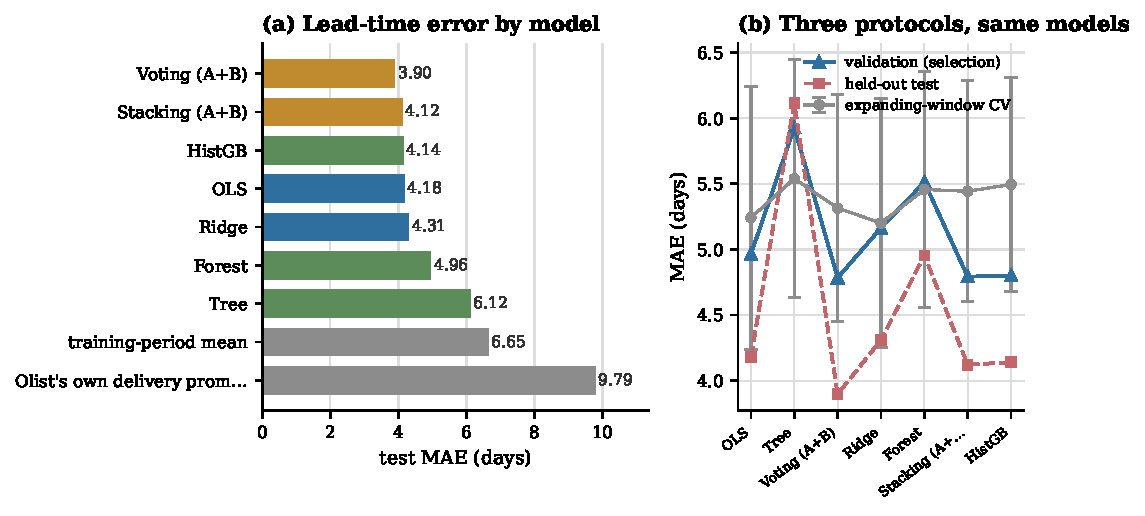
\includegraphics[width=\linewidth]{fig10_regression_ladder.pdf}
  \caption{Lead-time error by model, and the same models under three protocols.
  Panel (b) is the argument of Section~\ref{sec:cv}: expanding-window
  cross-validation does not order the candidates the way the validation period
  and the forward window --- which agree with each other --- do.}
  \label{fig:ladder}
\end{figure}

\begin{figure}[htbp]
  \centering
  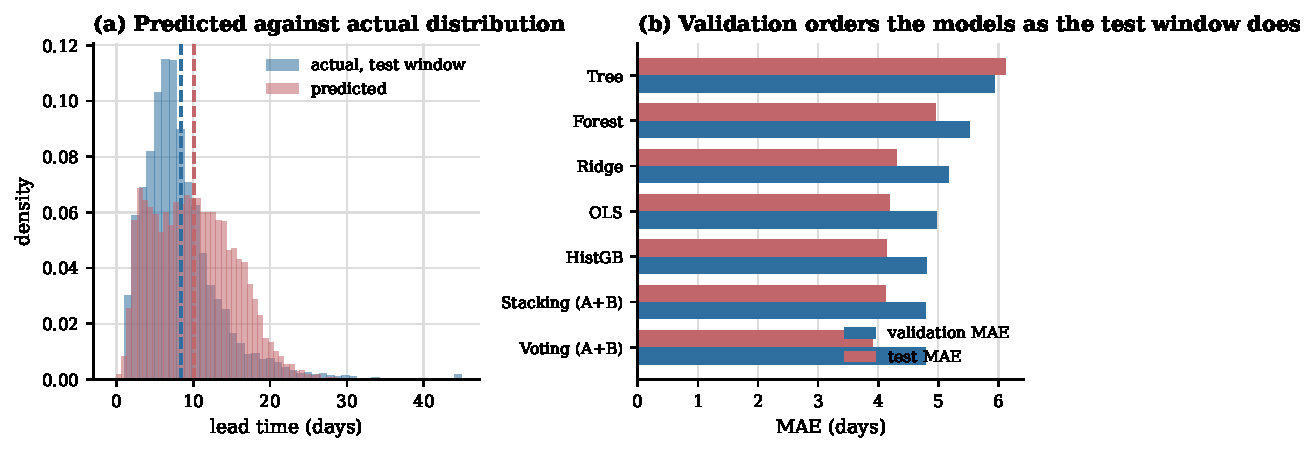
\includegraphics[width=\linewidth]{fig19_extrapolation.pdf}
  \caption{Why blending a linear model with a boosted one helps under drift. A
  tree cannot predict outside the range of the targets it was fitted on; lead
  times in the test window are systematically shorter than anything common in
  training. Panel (b) shows the validation period ordering the models as the test
  window does.}
  \label{fig:extrap}
\end{figure}

\begin{figure}[htbp]
  \centering
  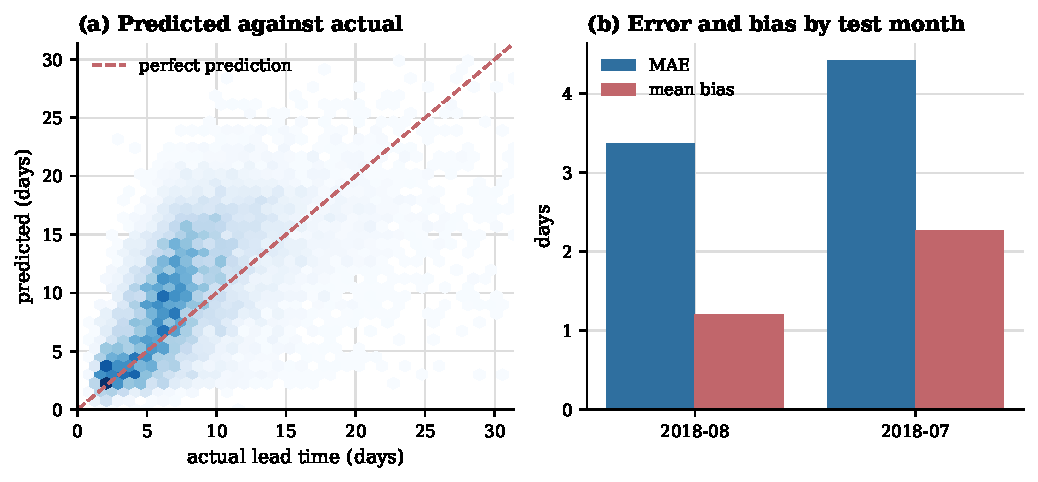
\includegraphics[width=\linewidth]{fig11_regression_residuals.pdf}
  \caption{Where the regression is wrong. The bias in panel (b) is positive in
  both test months: a model fitted on a slower past over-predicts how long a
  parcel will take.}
  \label{fig:resid}
\end{figure}

\begin{figure}[htbp]
  \centering
  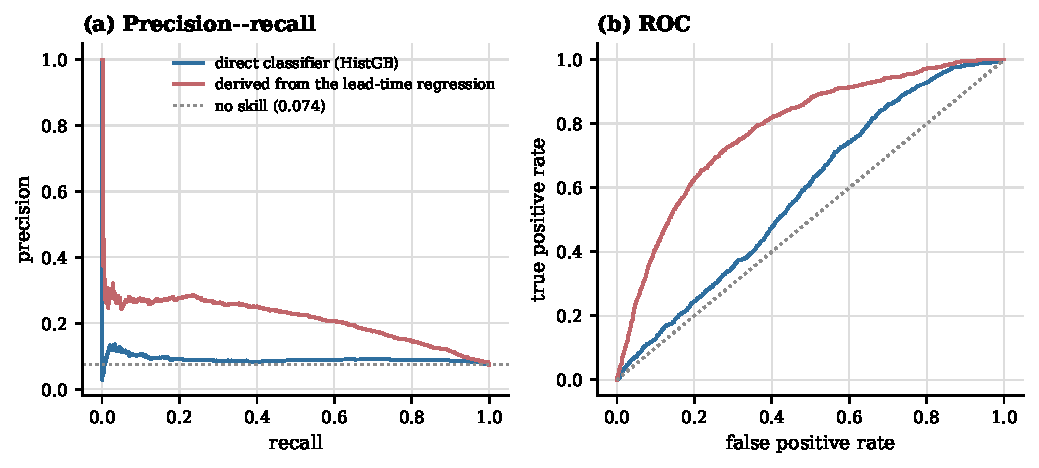
\includegraphics[width=\linewidth]{fig12_late_routes.pdf}
  \caption{Problem 1B. The flag derived from the lead-time regression against the
  best purpose-built classifier, on the forward test window.}
  \label{fig:routes}
\end{figure}

\begin{figure}[htbp]
  \centering
  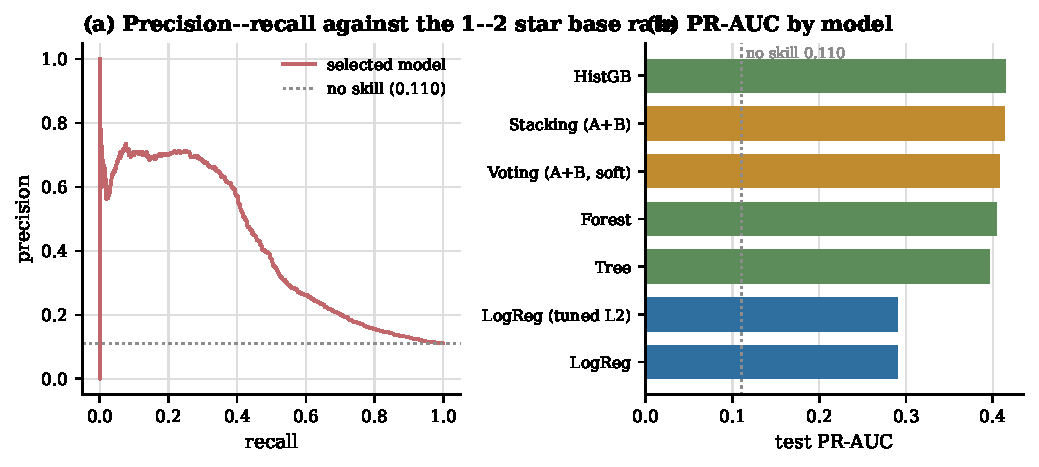
\includegraphics[width=\linewidth]{fig13_low_review.pdf}
  \caption{Problem 2 against its no-skill floor, and PR-AUC by model. Most of the
  achievable signal is already available from a single depth-limited tree.}
  \label{fig:lowreview}
\end{figure}

\begin{figure}[htbp]
  \centering
  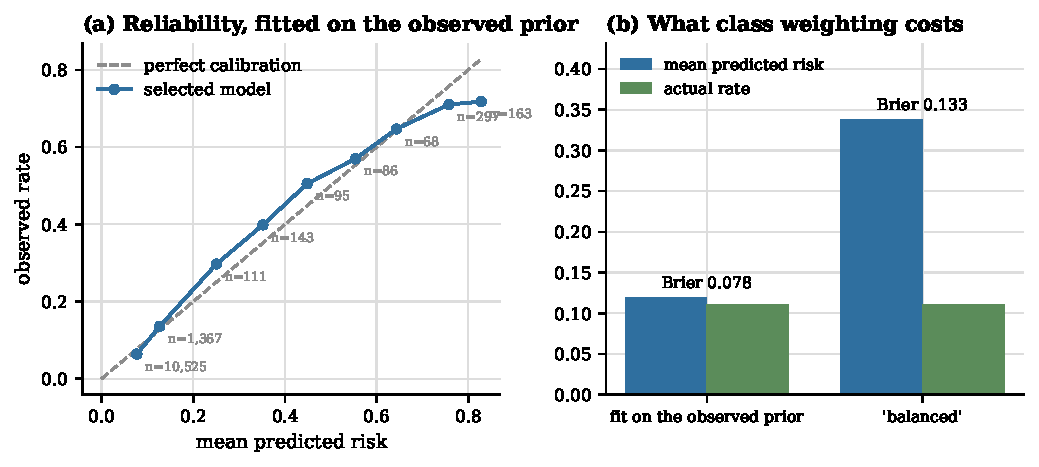
\includegraphics[width=\linewidth]{fig14_calibration.pdf}
  \caption{Calibration, and what class weighting costs. Weighting the loss leaves
  ranking unchanged and inflates mean predicted risk threefold against the actual
  rate.}
  \label{fig:calibration}
\end{figure}

\begin{figure}[htbp]
  \centering
  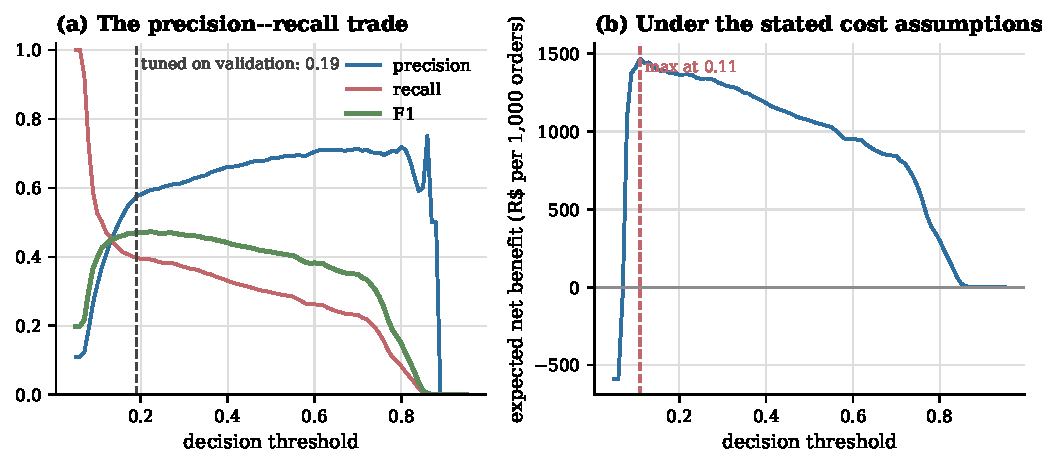
\includegraphics[width=\linewidth]{fig15_threshold_cost.pdf}
  \caption{Choosing the operating point for the review model, and what it is
  worth under the stated cost assumptions.}
  \label{fig:threshold}
\end{figure}

\begin{figure}[htbp]
  \centering
  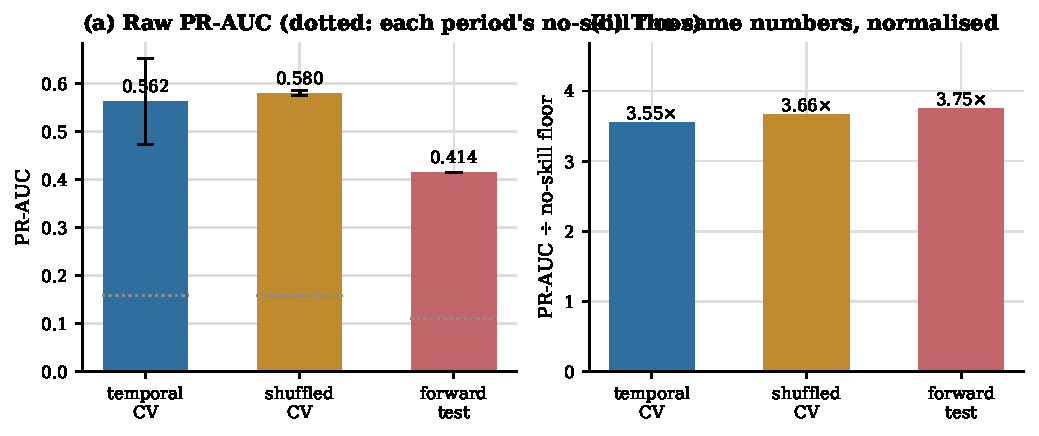
\includegraphics[width=\linewidth]{fig16_cv_protocol.pdf}
  \caption{One model, three protocols. Raw average precision disagrees across
  periods; divided by each period's no-skill floor the three agree to within 0.2
  of a multiple.}
  \label{fig:protocol}
\end{figure}

\begin{figure}[htbp]
  \centering
  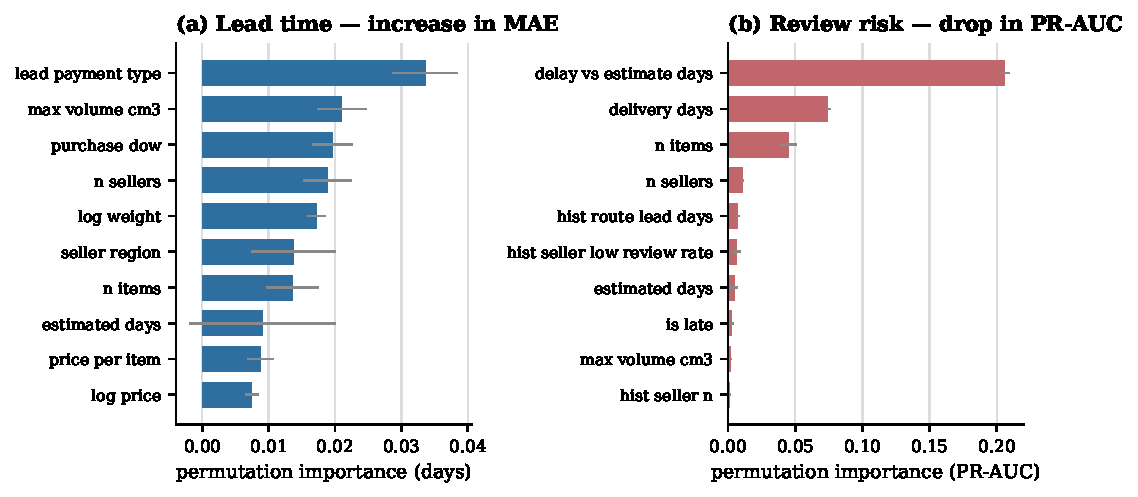
\includegraphics[width=\linewidth]{fig17_importance.pdf}
  \caption{Permutation importance on the test window. The review model rests on
  two features; the lead-time model on none in particular, which is a property of
  correlated predictors as much as of the model.}
  \label{fig:importance}
\end{figure}

\begin{figure}[htbp]
  \centering
  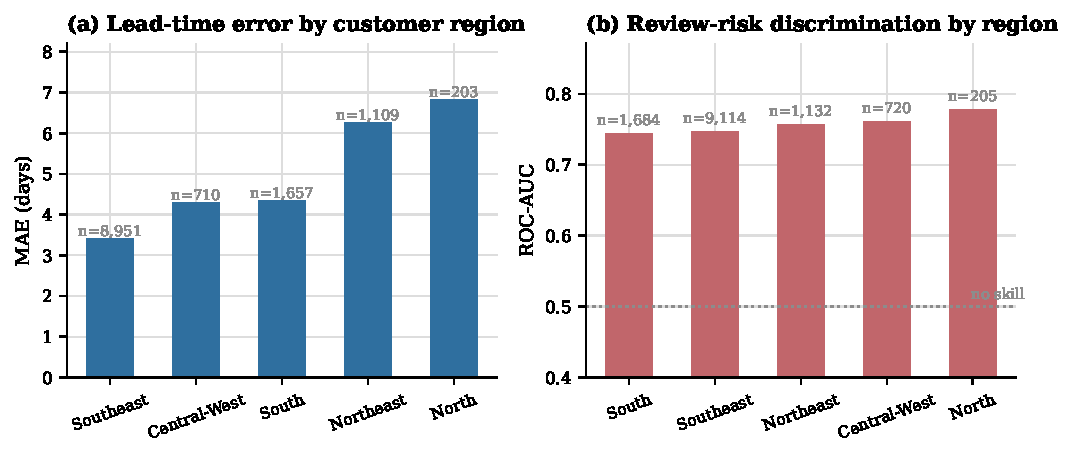
\includegraphics[width=\linewidth]{fig18_segments.pdf}
  \caption{Performance by customer region. The review model is stable across all
  five; the regression is not, and degrades exactly where deliveries are
  longest.}
  \label{fig:segments}
\end{figure}

\begin{figure}[htbp]
  \centering
  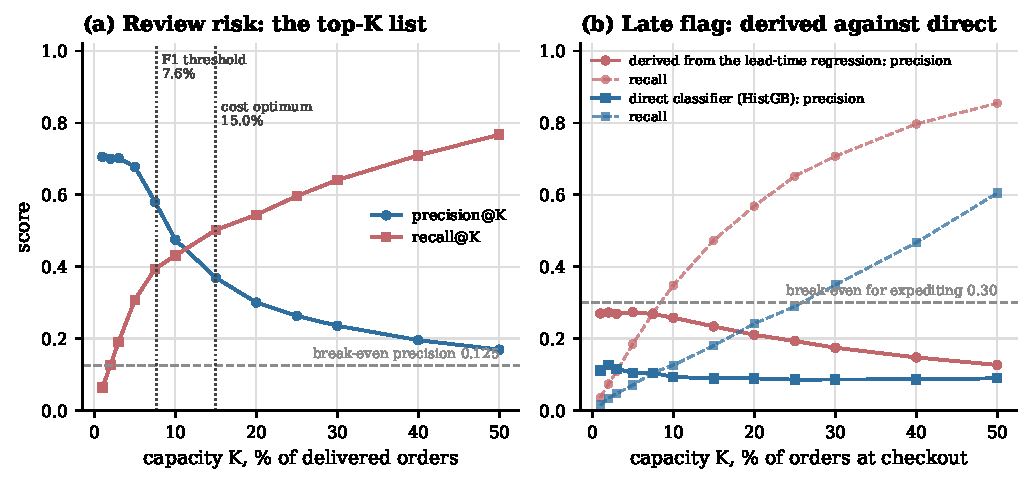
\includegraphics[width=\linewidth]{fig20_capacity.pdf}
  \caption{Precision and recall when only the top $K$ can be acted on
  (Section~\ref{sec:results-capacity}). (a) The review-risk list, with the
  report's two threshold operating points placed on the capacity axis; precision
  stays above the break-even at every capacity. (b) The late flag: the derived
  route beats the direct classifier at every $K$ and never reaches the
  break-even an expensive expedite would need.}
  \label{fig:capacity}
\end{figure}

\begin{figure}[htbp]
  \centering
  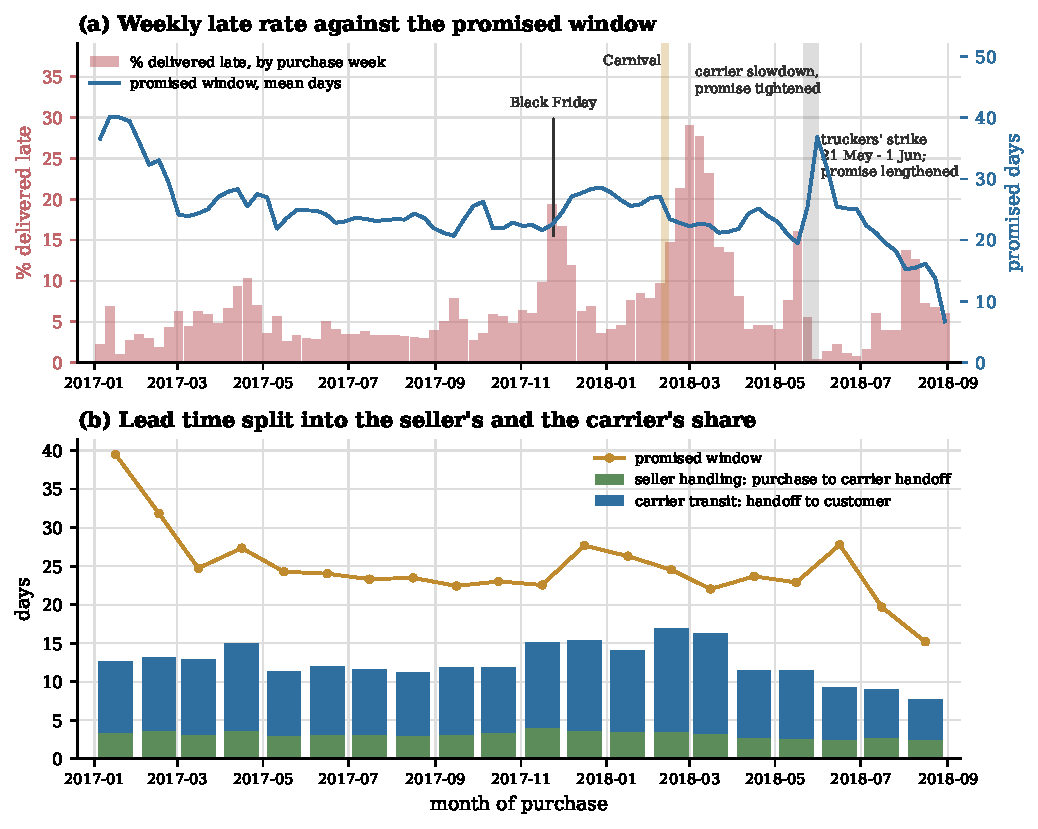
\includegraphics[width=\linewidth]{fig21_lateness_anatomy.pdf}
  \caption{Where the late deliveries came from (Appendix~\ref{app:lateness}).
  (a) Weekly late rate against the promised window: the February--March 2018
  peak coincides with a tightened promise, and the strike of 21 May--1 June 2018
  (shaded) hits the week promised before it, after which the promise is
  lengthened and the late rate collapses. (b) Lead time split at the carrier
  handoff: the peak is carrier transit, not seller handling.}
  \label{fig:lateness}
\end{figure}


% ============================== AI DECLARATION =============================
\clearpage
\section*{AI Tool Declaration}
\addcontentsline{toc}{section}{AI Tool Declaration}

We used OpenAI's ChatGPT and Anthropic's Claude to generate and validate ideas,
improve expression and refine our writing. We also used the models to debug our
code. All analytical decisions, results and conclusions were reviewed and
verified by the team against the underlying data, and we are responsible for the
content and quality of the submitted work.

\end{document}
